\chapter{Asking A 27 Year Old How to Make \$300 Million}

This lecture is an interview rather than a blackboard derivation, but it still has a definite mathematical spine. Scale is treated as a threshold problem, poverty as an environment problem, networking as a value-exchange problem, and wealth as a capital-deployment problem. No validated lecture screenshots survive for this chapter, so the equations and schematics below are not transcriptions of a board; they are careful codifications of the spoken argument.

\section{Scale, Stakes, and Backstory}

The lecture begins by forcing us to look at magnitude before explanation. We are told that the business did roughly \$149 million in the prior year and is projected to do about \$300 million in the present year. Only after that does the narration rewind into poverty, immigrant parents, and the decision to master sales. The order matters. We first see the scale, and only then do we ask what structure could possibly produce it.

Let us isolate the opening numerical anchors:
\begin{align}
R_{\text{last}} &= \$149\text{M},\\
R_{\text{proj}} &\approx \$300\text{M}.
\end{align}
From these, the interviewer's paraphrase is naturally formalized as
\begin{equation}
g=\frac{R_{\text{proj}}}{R_{\text{last}}}\approx \frac{300}{149}\approx 2.0.
\end{equation}
So the spoken claim is not merely that the company is large, but that it is on roughly a doubling trajectory. We should be careful here: these are company-scale figures, not clearly stated personal earnings.

The biographical rewind then adds the variables that the lecture wants us to keep in play: early scarcity, first-generation immigrant parents, the move into sales at eighteen, and the later transition from salesperson to sales leader to owner. In the lecture's own pacing, this is not sentimentality. It is the first constraint on the later theory. We are not being offered advice from a neutral perch; we are being shown a trajectory from low initial conditions to high commercial scale.

The operational snapshot of the present company is also concrete: more than 600 W2 employees, more than 3,000 sales reps selling through the firm, and a position among the large residential solar installers in the United States. The lecture's first claim, then, is that very large scale is real and must be explained structurally.

\section{From Seven Figures to Nine Figures}

The first serious mechanism of the lecture appears when the interviewer asks what carries a firm from seven to eight to nine figures. The answer is not a generic exhortation to work harder. It is a threshold model: different scales require different dominant constraints to be solved.

We may summarize the spoken ladder as
\begin{align}
\mathcal{S}_7 &= \{\text{idea},\text{sales},\text{marketing}\},\\
\mathcal{S}_8 &= \mathcal{S}_7 \cup \{\text{team}\},\\
\mathcal{S}_9 &= \{\text{product},\text{marketing},\text{sales},\text{team},\text{systems}\}.
\end{align}
The transcript briefly duplicates part of the line about team, but the intended classification is clear: seven figures demand a viable offer and the ability to sell it; eight figures demand people; nine figures demand documented systems.

\begin{figure}[h]
\centering
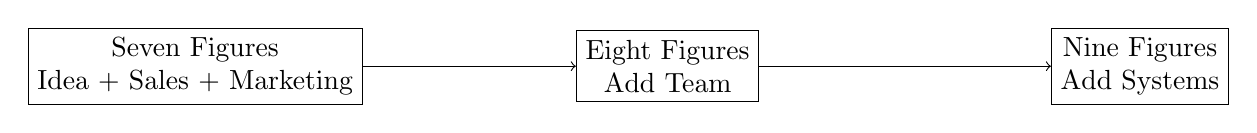
\begin{tikzpicture}
\node[draw, rectangle, align=center] (a) at (0,0) {Seven Figures\\Idea + Sales + Marketing};
\node[draw, rectangle, align=center] (b) at (6,0) {Eight Figures\\Add Team};
\node[draw, rectangle, align=center] (c) at (12,0) {Nine Figures\\Add Systems};
\draw[->] (a) -- (b);
\draw[->] (b) -- (c);
\end{tikzpicture}
\caption{Transcript-derived schematic of the lecture's scale thresholds.}
\end{figure}

The lecturer does not treat these as decorative additions. He treats them as bottleneck changes. To move from one scale to the next, we do not merely enlarge what we already have; we remove a new limiting factor.

\subsection{Question \& Answer}

\paragraph{Question.} Why do firms so often stall between eight figures and nine figures?

\paragraph{Answer.} Because an eight-figure firm can still be secretly organized around the founder. It may have sales, team, and activity, but its critical functions still terminate in one person. The nine-figure transition happens when the business becomes executable through procedures rather than personality.

We can formalize the lecture's operational intuition.

\begin{definition}
A business is founder-dependent if there exists a critical function \(f\) for which the founder is the only reliable operator.
\end{definition}

Let \(D(f)\in\{0,1\}\) denote whether function \(f\) is documented in a usable standard operating procedure. Then the lecture's point is that documentation creates transferability:
\begin{equation}
D(f)=1 \;\Rightarrow\; \exists\,c\neq o \text{ such that } c \text{ can execute } f,
\end{equation}
where \(o\) is the original operator and \(c\) is a colleague.

\begin{proposition}
As documentation coverage rises across critical functions, founder dependence falls.
\end{proposition}

\begin{proof}
If a critical function is undocumented, the absence of the founder or original operator may halt the function entirely. If the function is documented and the documentation is usable, another colleague can execute it in the founder's absence. Repeating this across more and more critical functions shifts execution from a single person to the machine of the business itself. In the lecture's language, the firm ceases to rely on the CEO and begins to rely on the system.
\end{proof}

This gives us a compact monotonic rule:
\begin{equation}
D_{\text{coverage}}\uparrow \;\Rightarrow\; \text{founder dependence}\downarrow.
\end{equation}
The force of the lecture lies in the extremity of the test: if the founder disappears, does the business continue to scale? The answer, for the nine-figure firm, is supposed to be yes.

\section{Escaping Poverty by Changing Environment}

The lecture then pivots from the architecture of firms to the architecture of personal escape. The interviewer asks what someone stuck in poverty should do, and the answer is sharper than a moral sermon. The lecturer's claim is that environment changes what one sees, whom one meets, and what becomes thinkable.

The heuristic can be written as
\begin{equation}
E[\text{opportunity access}] \propto \rho_{\text{wealth}}(\text{environment}),
\end{equation}
where \(\rho_{\text{wealth}}\) stands for the local density of capital, wealthy actors, and visible economic motion.

This is not a measured law. It is a transcript-backed heuristic. The lecture makes the point through strong contrasts. In one environment, everyone nearby earns ordinary wages, the surroundings are decayed, and daily life is demotivating. In another, one moves through a city full of expensive cars, active businesses, celebrities, and people with capital. The lecturer's claim is that the second setting changes both access and ambition.

He makes the point with a concrete, though plainly rhetorical, example: within a 30-mile radius of a major city, one may be near 14 billionaires and tens of thousands of multimillionaires. We should not elevate those numbers into audited statistics. Their function in the lecture is to model density. The essential statement is that proximity to concentrated money changes the expected set of opportunities one can encounter.

The transition is important. We have moved from systems inside the firm to fields of opportunity outside the firm. The hidden symmetry is that both arguments are about removing bottlenecks. In the business section, the bottleneck is the founder. In the poverty section, the bottleneck is environment.

\section{Investing in Self and in Position}

Once the lecture has argued that environment matters, it sharpens the claim into a priority rule. If someone is poor or living paycheck to paycheck, the first task is not prestige consumption and not even conventional investing in passive assets. The first task is to save enough to move and to build monetizable skill.

The lecture's spoken ordering is approximately this:
\begin{enumerate}
\item acquire skill, especially sales and marketing;
\item save enough to change environment;
\item postpone prestige spending;
\item delay passive asset investing until mobility and earning power have been strengthened.
\end{enumerate}

The interview does not present this as financial orthodoxy. It presents it as escape velocity. Let \(H\) denote human capital and \(P\) denote positional leverage created by relocation. Then the lecture's early-stage ordering can be summarized as
\begin{equation}
H + P \succ A_{\text{passive}},
\end{equation}
where \(A_{\text{passive}}\) stands for early passive asset accumulation.

Again, this is a reconstruction, not a board equation. The point is that a young person with weak income and weak surroundings may gain more by becoming a competent salesperson or marketer and moving into a richer economic field than by making symbolic passive investments while remaining trapped in place.

The lecture is especially emphatic here about motivation. Daily surroundings are not treated as decorative. They are treated as repeated inputs into ambition. A city full of moving business, visible wealth, and active deal flow becomes a machine for reminding us what is possible. The small dead environment, by contrast, becomes a machine for lowering our horizon.

\section{Sponsor Interlude}

At this point the transcript pauses for a sponsor message. For the purposes of the notes, we preserve the place of the interruption because the lecture resumes afterward on a new conceptual axis, namely relationships and social capital. But the sponsor copy does not belong to the chapter's main line of argument, so we do not let it carry analytic weight.

\section{Networking as Value Exchange}

After the interruption, the lecture returns with a question about relationships, networking, and the right people. The answer is deliberately harsh. Successful people do not ordinarily adopt strangers out of pure benevolence. They focus on what adds value to their own lives and work.

This is the lecture's social analogue of the systems argument. Just as a firm must not depend on personality without procedure, a person must not imagine access without value. The lecturer's own explanation can be summarized in a simple way: room-entry is not the first event; self-construction is the first event.

A cautious formalization is
\begin{equation}
\text{relational access} \sim f(\text{value provided},\text{credibility},\text{trust}),
\end{equation}
with the warning that this is only a schematic rendering of the spoken idea.

The lecture also distinguishes two mistakes. The first is to ask too early. The second is to carry around a social environment that lowers one's own perceived caliber. The line about who we do not spend time with is as important as the line about who we do. If our surrounding group signals chaos, addiction, or stagnation, then even stronger people may hesitate to bring us into better rooms.

So the networking doctrine of the lecture has three parts:
\begin{enumerate}
\item build yourself until invitation becomes plausible;
\item when admitted, do not arrive as a petitioner;
\item curate the company you keep, because other people judge us partly by our social orbit.
\end{enumerate}

The lecture makes this vivid through the imagined case of randomly meeting a billionaire in the street. Even if the meeting happens, the encounter does not automatically become ongoing access. Without prior value, stature, or trust, there is no reason for the connection to deepen. In that sense, the meeting is not the capital. The prepared person is the capital.

\section{Capital, Sales, and the Meaning of Wealth}

The late lecture turns toward money itself, then to sales, and finally to a distinction between being rich and being wealthy. These are not separate themes. They are different faces of the same picture: what matters is not mere possession, but the organization of productive force.

\subsection{Capital at Work}

The most counterintuitive claim in the lecture is the injunction to spend money rather than hoard it. We must state this carefully. The lecturer does not mean indiscriminate consumption. He means deployment.

Let \(K_{\text{idle}}\) denote nonworking cash beyond operating needs, and let \(K_{\text{deployed}}\) denote capital reinvested into the business or into skill and earning power. Then the lecture's preference is
\begin{equation}
K_{\text{idle}}\downarrow,\qquad K_{\text{deployed}}\uparrow.
\end{equation}

The spoken analogy is a luxury car with no gasoline. Idle capital may look impressive, but it does not move the machine. The more serious content is this: excess cash can create complacency. Reinvestment, by contrast, increases the productive value of the business and forces the organization to keep generating cash rather than resting on a cushion.

\begin{remark}
This is not a universal theorem of finance. It is the lecturer's operating philosophy, stated from the standpoint of a growth-oriented founder whose main asset is the business itself.
\end{remark}

\subsection{Sales as Conviction}

The sales section is one of the cleanest places where the lecture invites formal compression. The speaker explicitly weights tactics at \(10\%\) and conviction at \(90\%\):
\begin{equation}
\text{Sales effectiveness} \approx 0.9\,C + 0.1\,T,
\end{equation}
where \(C\) denotes conviction in the product and \(T\) denotes tactics, scripts, and objection handling.

This should not be mistaken for a calibrated empirical model. It is a rhetorical weighting. But it does express the lecture's central belief: technical training matters, yet visible belief in the product matters much more.

The reasoning runs as follows.
\begin{enumerate}
\item Buyers detect enthusiasm, confidence, and sincerity.
\item These signals depend strongly on whether the seller actually believes in the offer.
\item Tactics can refine a pitch, but they cannot fully substitute for conviction.
\item Therefore a weaker technician with strong product belief may outperform a polished technician who inwardly doubts the product.
\end{enumerate}

In that sense, the lecture treats conviction as a hidden state variable that changes conversion without necessarily appearing in the script itself.

\subsection{Rich and Wealthy}

The last economic distinction in the lecture is the difference, in Zane's own vocabulary, between being rich and being wealthy:
\begin{equation}
\text{rich}\sim \$4\text{M}-\$10\text{M}/\text{yr},\qquad \text{wealthy}\gtrsim \$1\text{B}.
\end{equation}
We should not universalize these thresholds. They are personal labels, not canonical economic definitions. Still, they serve a useful structural purpose. High income is not the same thing as overwhelming asset depth.

The lecture's illustrative example concerns a person with a net worth of \$100 million contemplating a \$50 million yacht with annual carrying cost above \$12 million. The burden ratio is
\begin{equation}
\frac{\$12\text{M}}{\$100\text{M}}=0.12.
\end{equation}
So a single prestige asset can consume roughly \(12\%\) of net worth per year in operating cost alone. This is the explicit worked example of the chapter.

What is the conclusion? That a headline number, even a very large one, may be too thin if the associated assets are nonproductive. The lecture's notion of wealth is therefore not simply ``a lot of money.'' It is money already deployed across businesses, financial assets, real estate, and other vehicles in such a way that even extravagant expenditures do not meaningfully threaten the whole.

\subsection{Final Compression}

The lecture ends by compressing its advice into two maxims: learn sales and do not quit. By the end, these no longer sound like ordinary motivational slogans. They summarize the entire chapter.

Sales, in the lecture's usage, means much more than closing deals. It means learning how human beings decide, what they believe, and how value is communicated. Not quitting, meanwhile, is not merely stubbornness. It is persistence through long bottleneck removal: first the poverty bottleneck, then the environmental bottleneck, then the systems bottleneck, then the social bottleneck, and finally the capital-allocation bottleneck.

\section{Summary}

We may summarize the lecture as a sequence of threshold arguments. Scale begins with an offer and the ability to sell it, but it does not reach nine figures until execution is transferred from the founder to systems. Personal escape begins with skill, but it accelerates when environment changes the density of opportunity. Networking does not begin with asking; it begins with becoming valuable. Money is not treated as reassurance in storage, but as capital to be deployed. And sales is not reduced to technique, because conviction is presented as the deeper driver.

The numerical claims in the lecture remain concrete: approximately \$149 million in prior-year revenue, approximately \$300 million projected, a roughly \(2\times\) growth multiple, a \(90/10\) rhetorical split between conviction and technique, and a \(12\%\) annual burden example for an expensive nonproductive asset. The larger point is that the lecture is not really about money in isolation. It is about the structure that allows money, teams, environment, and credibility to compound together.